\chapter{Testing}

\section{MPU}
In order to test the memory partition mapping, for an amount of space given, we use a non-specific initial
 pointer representing the begining of the memory free space, specific sizes for each partition and we
  write in each memory position the number of the partition that is ocupied with. In the end we print the
   whole memory avaiable for the test and confirm if the space given for each is enough and if they are
    allocated in the right place.\\
  If the amount of memory needed is bigger than the memory given a segmentation fault occurs.\\
 The tests cover the different partition memory distribuitions and sizes in memory, for the 3 cases of not
  having 1, 2 or  3 subregions used by the main partition of the region. For that we used 5 partitions, with
   specific memory requirements, in order to test the different memory alloctions combinations.\\
  The results printed showed us that the new sizes and subregions distribution allow us to have the less 
  spare memory possible, comparing with the theoretical calculations.\\
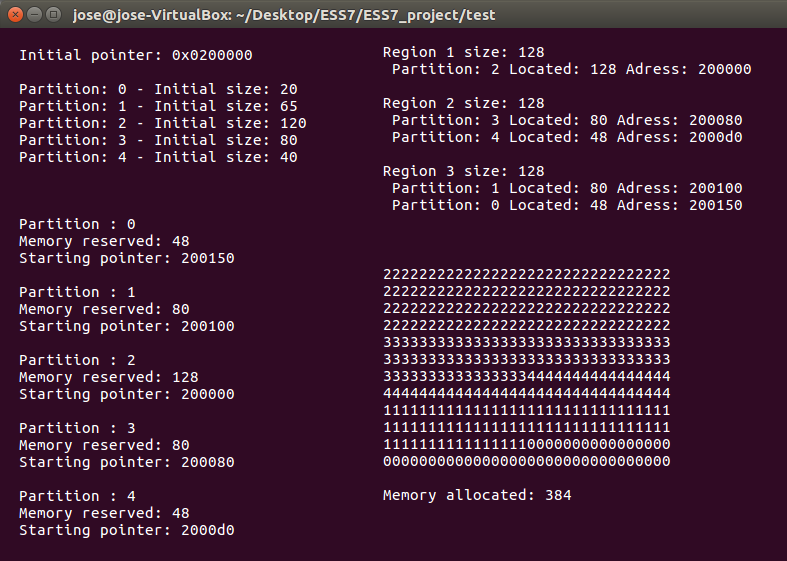
\includegraphics[width=15cm]{mpu_test.png} \\

\section{XML validation}

\section{Scheduler}

\section{ARINC Part 3}

\section{Message passing}

\section{The evil partition}